\documentclass[11pt]{article}
\usepackage[letterpaper,margin=1in]{geometry}
\usepackage{amsmath,amssymb,amsfonts}
\usepackage{booktabs,tabularx,array,multirow}
\usepackage{graphicx,float,caption}
\usepackage{xcolor}
\usepackage{microtype}
\usepackage{enumitem}
\usepackage{cite}
\usepackage[hidelinks]{hyperref}
\usepackage{url}
\usepackage{xspace}

\definecolor{cbadred}{HTML}{C0392B}
\definecolor{modelblue}{HTML}{2874A6}
\definecolor{softgray}{HTML}{F3F5F7}
\newcommand{\method}{MD-CBAD-DQN\xspace}
\newcommand{\R}{\mathbb{R}}
\DeclareMathOperator{\clip}{clip}

\title{\textbf{MD-CBAD-DQN: Model-Driven Counterfactual Bellman Advantage Distillation for Long-Term Satellite-Ground Task Scheduling}}
\author{
Bocheng Yang$^{1}$, Lujie Zheng$^{1}$, Jian Liu$^{1,2,*}$, and Bo Chen$^{1,*}$\\[3pt]
\small $^{1}$School of Aerospace, Harbin Institute of Technology (Shenzhen), Shenzhen 518055, China\\
\small $^{2}$Guangxi Key Laboratory of Precision Navigation Technology and Application,\\[-2pt]
\small Guilin University of Electronic Technology, Guilin 541004, China\\
\small $^{*}$Correspondence: liujian2024@hit.edu.cn; hitchenbo@hit.edu.cn
}
\date{}

\begin{document}
\emergencystretch=2em
\maketitle
\input{generated/reviewer_macros.tex}

\begin{abstract}
Satellite-ground scheduling is temporally coupled because a locally inexpensive action can consume resources needed by later tasks. A standard deep Q-network (DQN) nevertheless trains only the executed action, even when an analytical model can evaluate every one-step alternative. We introduce \method, which constructs model-based Bellman targets for all processing modes and distills their centered within-state advantages. In plain terms, training also asks what would have happened under the two unchosen processing modes; deployment uses no such preview. The factual target and factual loss term remain unchanged, while the total parameter update includes the auxiliary gradient. Tasks are generated from correlated data-volume and workload primitives; heat, energy, latency, and transmitted volume are derived from these primitives. Each learning method is trained with \IndependentModelSeeds{} independent model seeds and evaluated on shared traces in seven regimes and eight prespecified parameter envelopes. Against standard DQN, \method reduced mean cost by \PhysicalCBADMinPct--\PhysicalCBADMaxPct across all five fully coupled regimes. Paired intervals and Holm-adjusted sign tests were computed across model seeds. A four-step receding-horizon comparator and coupling controls delimit the claim. Analytical planning is preferable when coupling is absent or weak, whereas \method has the lowest mean cost among the evaluated deployment methods in all fully coupled regimes.
\end{abstract}

\noindent\textbf{Keywords:} satellite edge computing; task scheduling; model-driven reinforcement learning; counterfactual supervision; Bellman advantage distillation.

\begin{figure}[!htbp]
\centering
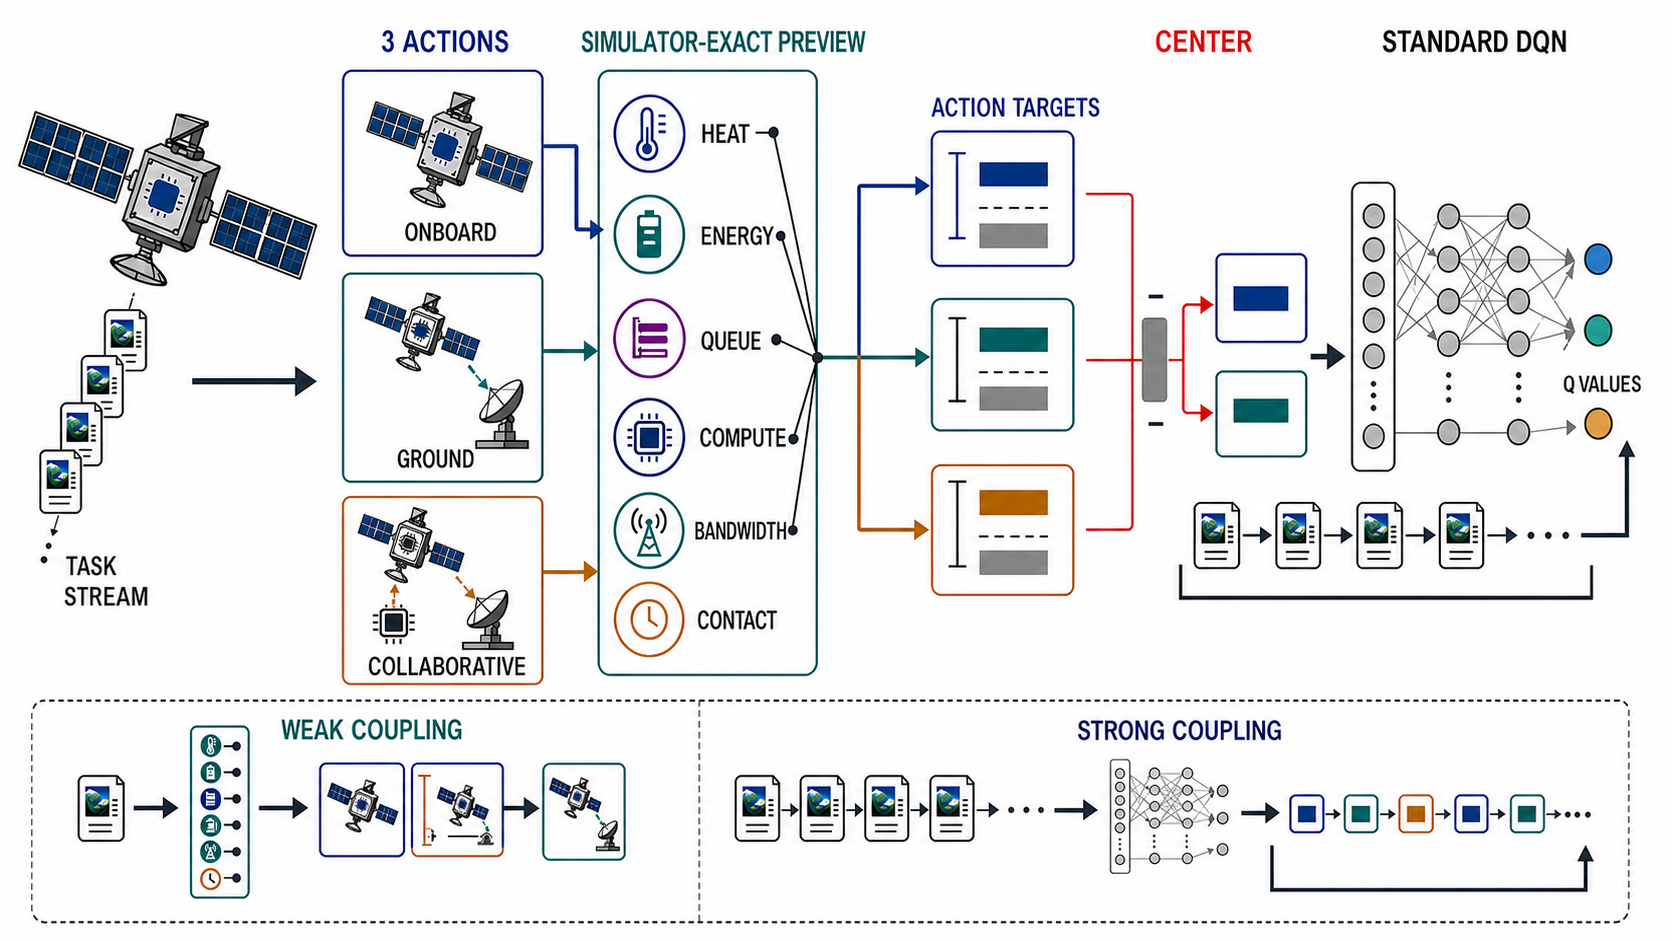
\includegraphics[width=0.98\textwidth,height=0.42\textheight,keepaspectratio]{figures/ai/fig_graphical_abstract_simulator_exact_arial.png}
\caption{Graphical overview of \method. Simulator-exact analytical previews expose the immediate cost and six post-action resources for all three scheduling actions. Centering the resulting Bellman targets isolates action-relative supervision. The factual standard-DQN target and loss term are retained, and the auxiliary loss contributes an additional gradient during training. The illustration is conceptual and encodes no quantitative results.}
\label{fig:graphical}
\end{figure}

\section{Introduction}

Earth-observation and communication satellites increasingly execute perception and decision workloads in orbit. Compact networks can reduce downlink demand and response latency under constrained onboard resources~\cite{9925218,10107454,10378728,10440355,10423050}. Yet onboard execution consumes heat, energy, and compute capacity, while ground offloading consumes contact time and bandwidth. A scheduler must therefore choose among onboard execution, complete offloading, and collaborative preprocessing.

Existing schedulers optimize constellation coordination, observation plans, service placement, deadlines, makespan, or energy use~\cite{RN8,RN9,RN10,RN20,RN22,RN23,RN27,RN28}. The present decision instead changes six resources that persist across task arrivals. These resources are heat, energy, queue occupancy, compute utilization, bandwidth, and remaining contact. Consequently, minimizing a known immediate cost need not minimize episode cost.

Standard DQN~\cite{mnih2015human,watkins1992q} learns one Bellman target from each factual tuple $(s_t,a_t,r_t,s_{t+1})$. Here, the resource equations can also evaluate every unexecuted action without advancing the environment or revealing later tasks. The unresolved question is how to use these simulator-exact alternatives while preserving a controlled standard-DQN comparison. Absolute counterfactual targets provide more supervision, but their common state-value offset does not affect action selection.

We address this question with \method. The method previews every action, forms standard target-network Bellman targets, and centers predicted and target values within each state. It then distills the resulting action advantages while the factual Huber loss anchors the absolute Q scale. Counterfactual previews are restricted to training.

Our contributions are:

\begin{enumerate}[leftmargin=1.6em]
    \item We formulate three satellite-ground processing modes as a 21-dimensional sequential problem and derive coupled heat, energy, latency, and transmission descriptors from common task primitives.
    \item We introduce centered counterfactual Bellman advantage distillation, which uses simulator-exact full-action outcomes to supervise the action gaps that determine scheduling decisions.
    \item We evaluate the complete centered full-action objective against a strictly matched standard-DQN backbone, then bound its performance with coupling controls and a four-step model-based planner across seven regimes and eight parameter envelopes.
\end{enumerate}

\section{Related Work and Novelty Positioning}

\subsection{Satellite-ground scheduling}

Satellite schedulers cover constellation coordination, observation planning, service placement, and energy-aware offloading~\cite{RN8,RN9,RN10,RN20,RN22,RN23,RN27,RN28}. Our setting combines an explicit cost for every action with resource carryover between task arrivals. The one-step objective is therefore observed rather than hidden. Learning is justified only when present actions change future feasibility.

\subsection{Model use and counterfactual learning}

Dyna established predicted experience for value learning and planning~\cite{sutton1991dyna}. Counterfactual data fusion and causal augmentation construct transitions under structural assumptions~\cite{forney2017counterfactual,armengol2024caiac}. Counterfactual credit assignment instead separates action influence from future randomness~\cite{mesnard2021counterfactual}. Recent work also studies multi-action generative interfaces and joint quantities across action outcomes~\cite{kaya2026joint}. Counterfactual information in reinforcement learning is therefore not new by itself.

Advantage learning widens action gaps through modified operators~\cite{bellemare2016gap}, whereas \method preserves the standard Bellman operator. It adds centered targets that are exact under the specified deterministic simulator but does not synthesize replay trajectories. Each alternative shares the current task and exogenous next task, while only six endogenous resources change. Our novelty claim is consequently narrow. We claim this full-action, centered auxiliary objective and its scheduling application, not counterfactual simulation or advantage learning in general.

\section{System Model and Immediate-Cost Quantification}
\label{sec:system}

At task arrival $t$, a satellite selects one of three actions:
\begin{equation}
\mathcal A=\{\alpha_s,\alpha_g,\alpha_{s\&g}\},
\end{equation}
where $\alpha_s$ executes onboard and downlinks the result, $\alpha_g$ downlinks the complete input for ground execution, and $\alpha_{s\&g}$ performs onboard preprocessing followed by ground execution.

\begin{figure}[H]
\centering
\includegraphics[width=0.98\textwidth,height=0.42\textheight,keepaspectratio]{figures/ai/fig_system_modes_arial.png}
\caption{Three satellite-ground processing pathways. Each arriving task is executed onboard, transferred for ground execution, or preprocessed collaboratively before ground completion. The analytical transition model returns the immediate cost and the post-action heat, energy, queue occupancy, compute utilization, bandwidth, and remaining contact.}
\label{fig:system}
\end{figure}

\subsection{Implemented immediate-cost model}

The revised experiments use the dimensionless linear cost implemented by the physical-consistency simulator. Let $x_k$ denote the 15 task descriptors in Table~\ref{tab:state_dictionary}. Each descriptor is normalized as
\begin{equation}
\bar x_k=\clip(x_k/s_k,0,1.5),
\end{equation}
where $s_k$ is the corresponding scale. For inherited normalized bandwidth $b$, the available return rate is $R(b)=2.2+217.8b$ Mbit s$^{-1}$. The three action latencies are
\begin{align}
L_s&=x_3+1000x_6/R(b),\notag\\
L_g&=x_8+1000x_9/R(b),\notag\\
L_{s\&g}&=1000x_{12}/4+x_{13}+1000x_{15}/R(b).
\label{eq:latencies}
\end{align}
The implemented immediate costs are
\begin{align}
c_s^{imm}={}&0.70\bar x_1+0.65\bar x_2+0.00045L_s+0.55\bar x_5
+0.35\bar x_6+0.35h+0.12(1-e),\notag\\
c_g^{imm}={}&0.45\bar x_7+0.00045L_g+0.55\bar x_9
+0.35(0.28-\tau)_+,\notag\\
c_{s\&g}^{imm}={}&0.55(\bar x_{10}+\bar x_{11})+0.55\bar x_{14}
+0.00045L_{s\&g}+0.45\bar x_{15}\notag\\
&+0.18h+0.12q+0.18(0.22-\tau)_+.
\label{eq:implemented_costs}
\end{align}
Here $h$, $e$, $q$, and $\tau$ are inherited heat, remaining energy, queue occupancy, and contact duration. The weights are fixed simulator assumptions rather than fitted mission utilities. They are applied identically during training, counterfactual preview, MPC evaluation, and deployment evaluation. Automated tests reproduce Eq.~\eqref{eq:implemented_costs} from the 15 raw descriptors and compare it with all three code outputs.

\begin{table}[H]
\centering
\caption{Implemented 15-dimensional task descriptor dictionary. The six appended resource coordinates are $h$, $e$, $q$, compute utilization $u$, bandwidth $b$, and contact duration $\tau$.}
\label{tab:state_dictionary}
\resizebox{\textwidth}{!}{\input{generated/table_state_dictionary.tex}}
\end{table}

\subsection{Physically coupled task and communication generator}

The revised simulator does not sample heat, workload, data volume, and latency independently. It first draws correlated latent variables $(v_t,w_t)$ with correlation parameter 0.68 and maps them through a logistic transform to raw data volume $D_t\in[8,64]$ Mbit and workload $W_t\in[0.25,4.0]$ GFLOP. Result and collaborative-feature volumes are
\begin{equation}
D_t^{res}=r_tD_t,\quad r_t\in[0.01,0.05],\qquad
D_t^{feat}=f_tD_t,\quad f_t\in[0.08,0.30].
\end{equation}
The implementation enforces $D_t^{res}\le D_t^{feat}\le D_t$. A workload-dependent fraction $p_t\in[0.20,0.45]$ is processed onboard in the collaborative mode. Given onboard and ground rates $R_s=4$ and $R_g=80$ GFLOP s$^{-1}$, processing time is derived as $W/R$, rather than sampled separately. Compute power rises monotonically from 4 to 20 W with workload; compute heat is 0.78 times compute energy. Transmission time is data volume divided by the effective return rate
\begin{equation}
R_t^{link}=2.2+217.8b_t\quad\text{Mbit s}^{-1},
\end{equation}
and transmission heat is 0.55 times transmit energy. These values are engineering envelopes, not fitted flight distributions. Their scale is consistent with the range of modern SmallSat computing-system power reported by NASA and with NASA ground-network examples spanning 2.2 Mbit s$^{-1}$ S-band to 220 Mbit s$^{-1}$ X-band returns~\cite{nasa2026avionics,nasa2026ground}. The bounded data-reduction factors represent the bandwidth-reduction role of onboard image compression, not a claim about one instrument-specific codec~\cite{ccsds122}. Table~\ref{tab:parameters} states every implemented assumption.

\begin{table}[H]
\centering
\caption{Physical primitives and provenance of the revised simulator. Values define a transparent engineering envelope; they are not presented as a fitted flight distribution.}
\label{tab:parameters}
\resizebox{\textwidth}{!}{\input{generated/table_parameter_provenance.tex}}
\end{table}

An automated audit generated \PhysicalAuditTasks{} tasks before training. All values were finite and positive, all data-flow inequalities held, and the empirical raw-data--workload correlation was \PhysicalCorrDataWork. Figure~\ref{fig:physical} shows the resulting dependence structure. Constant-rate columns have zero variance and are therefore excluded from correlation coefficients.

\begin{figure}[H]
\centering
\includegraphics[width=0.98\textwidth]{figures/fig_physical_generator.pdf}
\caption{Physical-consistency audit of the revised generator. (a) A legibility sample of 2,000 of 20,000 tasks; color encodes heat derived from compute energy. (b) Correlations computed from all 20,000 tasks. No fitted flight distribution is implied.}
\label{fig:physical}
\end{figure}

\section{Sequential Scheduling Formulation}
\label{sec:mdp}

\subsection{State and transition}

The normalized 21-dimensional state is
\begin{equation}
s_t=[x_t,z_t],\qquad z_t=[h_t,e_t,q_t,u_t,b_t,\tau_t],
\end{equation}
where $x_t\in\R^{15}$ contains the task inputs defined in Table~\ref{tab:state_dictionary}. The six resource variables denote normalized heat, remaining energy, queue occupancy, compute utilization, bandwidth, and contact duration.

Executing action $a_t$ changes resources before the next exogenous task arrives. The implemented transition is
\begin{align}
h_{t+1}&=\clip(0.86h_t+0.17c\widehat Q_t^{(a_t)},0,1.3),\notag\\
e_{t+1}&=\clip(e_t+0.006-c\Delta e_t^{(a_t)},0,1),\notag\\
q_{t+1}&=\clip(q_t+c(\Delta q_t^{(a_t)}-\mu_t^{(a_t)}),0,1.3),\notag\\
u_{t+1}&=\clip(0.68u_t+0.32c\widehat w_t^{(a_t)},0,1.2),\notag\\
b_{t+1}&=\clip(\bar b_{t+1}-c\ell_t^{(a_t)},0.08,1),\notag\\
\tau_{t+1}&=\clip(\bar\tau_{t+1}-0.10c\widehat B_t^{(a_t)},0.05,1).
\label{eq:transition}
\end{align}
Here $\widehat Q$, $\widehat w$, and $\widehat B$ are normalized action-specific heat, work, and data demands. The terms $\Delta e$, $\Delta q$, $\mu$, and $\ell$ denote deterministic resource-use, queue, service, and link-occupation functions. Their implementations are provided with the simulator. Exogenous link variables $\bar b$ and $\bar\tau$ are sampled before each episode. Coupling $c=0$ removes action-dependent carryover, $c=0.5$ weakens it, and $c=1$ defines full coupling.

\subsection{Reward and standard DQN backbone}

The reward is the negative immediate cost plus post-decision feasibility penalties:
\begin{align}
r_t={}&-c_t^{imm}-c\big[12(h_{t+1}-0.78)_+ +15(0.18-e_{t+1})_+\notag\\
&+8(q_{t+1}-0.75)_+ +10\mathbf 1_{a_t\ne\alpha_s}(0.14-\tau_t)_+\big].
\label{eq:reward}
\end{align}
The DQN uses the unmodified factual target
\begin{equation}
y_t=r_t+\gamma(1-d_t)\max_{a'}Q_{\bar\theta}(s_{t+1},a'),
\label{eq:factual}
\end{equation}
and factual loss
\begin{equation}
L_{DQN}=\mathcal H\big(Q_\theta(s_t,a_t),y_t\big),
\end{equation}
where $\mathcal H$ denotes the Huber loss. The target network both selects and evaluates the maximizing action, as required by standard DQN.

\section{Model-Driven Counterfactual Bellman Advantage Distillation}
\label{sec:method}

The proposed method preserves the factual DQN target and factual loss term and adds one training-only auxiliary path. This path supplies targets for unexecuted actions and removes their shared within-state offset. The experiment evaluates this complete auxiliary objective rather than attributing performance to either operation in isolation.

\subsection{Side-effect-free full-action preview}

For every replayed factual state, the analytical transition evaluates each $a\in\mathcal A$:
\begin{equation}
(\tilde \ell_{t,a},\tilde z'_{t,a})=F_{preview}(x_t,z_t,a).
\end{equation}
Here $\tilde \ell_{t,a}$ contains the immediate cost and post-decision feasibility penalty for action $a$. The preview does not advance time, mutate state, alter trajectories, or consume random numbers. It also reads no task beyond $x_{t+1}$. All alternatives share that next task and the exogenous link trace. The counterfactual next state therefore replaces only the six endogenous resource coordinates:
\begin{equation}
\tilde s'_{t,a}=[x_{t+1},\tilde z'_{t,a}].
\end{equation}
Evaluation and deployment never call the preview interface.

\subsection{All-action counterfactual Bellman targets}

The simulator-exact one-step outcome yields
\begin{equation}
\tilde y_{t,a}=-\tilde \ell_{t,a}+\gamma(1-d_t)
\max_{a'}Q_{\bar\theta}(\tilde s'_{t,a},a').
\label{eq:cf_target}
\end{equation}
The targets create no multi-step rollout and insert no counterfactual transition into replay. They are used only after state-wise centering in the complete method below.

\subsection{Centered advantage distillation}

Absolute targets in Eq.~\eqref{eq:cf_target} share a bootstrapped state-value offset. Deployment selects $\arg\max_a Q(s,a)$, so a common additive offset cannot change the action. We define predicted and target centered advantages as
\begin{align}
\widehat A_{t,a}&=Q_\theta(s_t,a)-\frac{1}{|\mathcal A|}\sum_jQ_\theta(s_t,j),\notag\\
\tilde A_{t,a}&=\tilde y_{t,a}-\frac{1}{|\mathcal A|}\sum_j\tilde y_{t,j}.
\label{eq:center}
\end{align}
The advantage and total losses are
\begin{align}
L_{adv}&=\frac{1}{|\mathcal A|}
\sum_{a\in\mathcal A}\mathcal H(\widehat A_{t,a},\tilde A_{t,a}),\notag\\
L_{CBAD}&=L_{DQN}+\lambda L_{adv}.
\label{eq:cbad}
\end{align}
The factual term anchors the absolute Q scale, while $L_{adv}$ teaches all action gaps. The only added algorithmic hyperparameter is $\lambda$.

\begin{figure}[H]
\centering
\includegraphics[width=0.98\textwidth,height=0.43\textheight,keepaspectratio]{figures/ai/fig_cbad_mechanism_simulator_exact_arial.png}
\caption{Training-only CBAD mechanism. The upper path retains the factual standard-DQN target and Huber loss. The lower path previews all three actions, constructs three Bellman targets, centers them within state, and distills their relative advantages. Both losses update the online Q-network; the target network is synchronized only at the shared fixed interval. Preview outputs are unavailable during evaluation and deployment.}
\label{fig:mechanism}
\end{figure}

\begin{figure}[H]
\centering
\fbox{\begin{minipage}{0.93\textwidth}
\textbf{Algorithm 1: Pure-DQN training with CBAD}
\begin{enumerate}[leftmargin=1.6em,itemsep=2pt,topsep=4pt]
\item Initialize uniform replay $\mathcal D$, online $Q_\theta$, and target $Q_{\bar\theta}\leftarrow Q_\theta$.
\item At each real step, observe $s_t$ and preview $(\tilde \ell_{t,a},\tilde z'_{t,a})$ for all actions without side effects.
\item Select $a_t$ by the shared epsilon-greedy schedule, execute it once, and store the factual tuple plus previews.
\item When an update is due, sample one uniform mini-batch, compute the factual loss, compute Eqs.~\eqref{eq:cf_target} and \eqref{eq:center}, and update $\theta$ using Eq.~\eqref{eq:cbad}.
\item Synchronize $Q_{\bar\theta}$ at the shared fixed interval.
\end{enumerate}
\end{minipage}}
\par\smallskip
\caption*{Training previews are never used for evaluation or deployment.}
\label{alg:cbad}
\end{figure}

\section{Experimental Design and Settings}
\label{sec:experiments}

\subsection{Design principles}

The design separates two questions. Standard DQN versus CBAD tests the complete centered counterfactual objective against an unchanged factual DQN backbone. Coupling controls and MPC-4 test whether long-horizon learning remains useful after delayed resource effects are weakened or removed.

Standard DQN and CBAD share every component except the centered counterfactual auxiliary objective. They use the same input, network, target, replay, exploration, optimizer, update cadence, target synchronization, and gradient clipping. The implementation excludes Double DQN, dueling networks, prioritized replay, multi-step returns, noisy networks, and distributional value learning.

Calibration and confirmation use disjoint model seeds and test-trace namespaces. Calibration considered $\lambda\in\{0.1,0.3,1,3\}$ with model seeds 700--703. It selected and locked $\lambda=0.3$. Confirmation used seeds 800--819 without post hoc removal, replacement, or selection. Every learned policy was trained only on the nominal $c=1$ distribution.

\begin{figure}[!htbp]
\centering
\includegraphics[width=0.98\textwidth,height=0.42\textheight,keepaspectratio]{figures/ai/fig_experiment_protocol_20seeds_arial.png}
\caption{Locked calibration-confirmation protocol. Four calibration seeds compare $\lambda\in\{0.1,0.3,1.0,3.0\}$, after which $\lambda=0.3$ and the configuration are frozen. Twenty disjoint confirmation seeds, 800--819, are each evaluated on 20 paired traces in seven regimes, with no confirmatory tuning or seed exclusion.}
\label{fig:protocol}
\end{figure}

\subsection{Training configuration}

Each network has 21 inputs, hidden widths 128--128--64, ReLU activations, and three outputs. Every model receives 600 episodes of 64 tasks, totaling 38,400 real interactions. Fixed settings are $\gamma=0.97$, learning rate $3\times10^{-4}$, batch size 128, replay capacity 100,000, and gradient-norm limit 10. Training begins after 128 transitions and performs one update every four interactions. The checkpoint field \texttt{target\_interval=250} is evaluated only on update calls; because updates occur at interaction counts divisible by four, the two divisibility conditions coincide every 500 real interactions. Epsilon decreases linearly from 1 to 0.05 over 13,440 interactions.

The contextual bandit uses the same network, optimizer, exploration schedule, and interaction budget, with $\gamma=0$. It therefore learns the modeled one-step reward without a long-horizon Bellman term. Uniform replay stores only one-step factual transitions, with preview outputs attached as auxiliary training data.

All reported reviewer-revision experiments use the physically coupled generator described above. Link bandwidth and contact follow bounded noisy periodic traces generated at reset. Burst and thermal-stress episodes multiply raw data and workload by 1.45 during one contiguous interval; all dependent heat, energy, latency, and transmission quantities are recomputed from those primitives. The original independently sampled generator is retained only as a historical reproducibility mode and is not used for the revised results.

\subsection{Seven evaluation regimes}

The seven regimes separate coupling controls from fully coupled operating conditions:

\begin{enumerate}[leftmargin=1.6em]
    \item \textbf{Static ($c=0$):} removes action-dependent state transitions and delayed penalties.
    \item \textbf{Reduced coupling ($c=0.5$):} halves action-dependent resource effects.
    \item \textbf{Nominal ($c=1$):} matches the fully coupled training distribution.
    \item \textbf{Burst:} increases contiguous compute and thermal demand.
    \item \textbf{Link-limited:} reduces the available bandwidth trace by 0.22 before clipping.
    \item \textbf{Energy-limited:} lowers initial energy from 0.88 to 0.62.
    \item \textbf{Thermal-stress:} raises initial heat from 0.22 to 0.42 and includes the burst interval.
\end{enumerate}

The first two regimes control temporal coupling. The remaining five retain full coupling. Models trained at $c=1$ are transferred to both controls without retraining. Their control performance therefore measures a boundary and transfer mismatch, rather than the best policy attainable at lower coupling.

\subsection{Planning comparator, outcomes, and inference}

The deployment comparison includes immediate-cost argmin, a contextual bandit, a resource-threshold heuristic, standard DQN, \method, and an exhaustive short-horizon model-based planner. At every real decision, the planner enumerates all $3^H$ action sequences over the next $H=4$ known tasks and link states, minimizes the discounted modeled cost with $\gamma=0.97$, executes only the first action, and replans. It is exact for this four-step perfect-forecast objective but is not a 64-step global optimum; exhaustive enumeration of the complete episode would require $3^{64}$ sequences. This comparator therefore tests whether a conventional rolling planner resolves the sequential problem at practical depth while exposing its forecast and computation assumptions. Fixed onboard and fixed ground policies serve as supplemental controls.

The primary outcome is episode total cost. Secondary outcomes are immediate cost, delayed penalty, energy use, modeled latency, transmitted data, threshold-exposure steps, action fractions, planner wall-clock time, maximum heat, and minimum remaining energy. Every policy uses the same 20 evaluation traces within each model seed. Traces are averaged within each independently trained seed, so the independent unit is the model seed ($n=20$ per learning method). Two-sided 95\% percentile intervals use 10,000 paired bootstrap resamples with seed 20260829. Exact two-sided paired sign tests evaluate directional consistency, with Holm adjustment across the five fully coupled primary comparisons. We also report every seed-level difference and the range of leave-one-seed-out mean effects. Test traces and bootstrap resamples are not treated as independent units.

\subsection{Prespecified sensitivity and training diagnostics}

Without retraining or selecting models, the nominal evaluation was repeated under eight profiles: the reference configuration; compute demand $\pm20\%$; raw data volume $\pm20\%$; energy use $+20\%$; heat load $+20\%$; and link capacity $-20\%$. Each profile retained the same 20 models, 20 paired traces per seed, and inference rule, with Holm adjustment across the eight profiles. Training logs record every episode for all 20 seeds. Curves report a causal 25-episode moving mean and seed-level mean $\pm$ SD for total cost, energy use, latency, and delayed penalty. These diagnostics describe optimization trajectories; confirmation claims remain based on held-out traces.

\subsection{Preview-model misspecification test}

The main experiment assumes that the analytical preview matches the simulator transition. To test this dependence, two additional CBAD model sets were trained without changing the factual environment or deployment evaluation. One set scaled preview one-step costs (immediate cost plus modeled penalty) and action-induced resource changes by 0.85, while the other used 1.15. Resource predictions were clipped to the same physical bounds after scaling around the current resource state. Each condition used the same 20 seeds, training budget, network, replay, and evaluation traces as the main experiment. These scales were fixed as symmetric stress tests and were not used for model selection.

\subsection{Reproducible result entry point}

The unique reviewer-revision entry point is \texttt{python -m md\_cbad\_dqn.reviewer\_experiments all --seeds 800-819 --resume}. It trains or loads 60 primary learned-policy checkpoints, evaluates eight deployment policies on $7\times20\times20=2{,}800$ shared seed--trace settings (22,400 raw rows), evaluates four policies in eight sensitivity profiles (12,800 rows), and evaluates four policies in five regimes for the preview-error study (8,000 rows). The run writes the resolved configuration, environment and package versions, checkpoint and result hashes, finite-value checks, and expected row counts to a machine-readable validation manifest. Table and figure scripts consume these result files directly.

\section{Results}
\label{sec:results}

\subsection{Physical consistency preserves the CBAD--DQN effect}

Table~\ref{tab:main} and Fig.~\ref{fig:seven} summarize the revised primary outcome. Values are mean $\pm$ SD across 20 independent model seeds after averaging 20 shared traces within each seed.

\begin{table}[H]
\centering
\caption{Episode total cost for deployment comparators under the physically coupled generator. MPC-4 is exact only for its stated four-step perfect-forecast objective. Lower is better; bold marks the lowest mean.}
\label{tab:main}
\resizebox{\textwidth}{!}{\input{generated/table_reviewer_main.tex}}
\end{table}

\begin{figure}[H]
\centering
\includegraphics[width=0.98\textwidth]{figures/fig_reviewer_primary.pdf}
\caption{Seven-regime performance under physically coupled task generation. Error bars are SD across 20 independent model seeds after within-seed trace averaging. The ordinate changes between the coupling-control and fully coupled panels.}
\label{fig:seven}
\end{figure}

\begin{table}[H]
\centering
\caption{Seed-level primary inference for CBAD minus standard DQN in the five fully coupled regimes. Negative differences favor CBAD. The Holm family contains these five prespecified comparisons. LOO denotes the range of leave-one-seed-out mean differences.}
\label{tab:primary_inference}
\resizebox{\textwidth}{!}{\input{generated/table_primary_inference.tex}}
\end{table}

\begin{figure}[H]
\centering
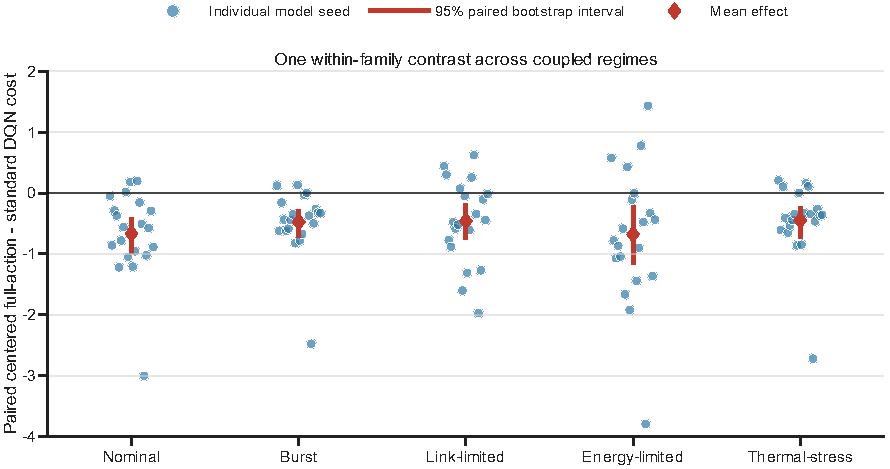
\includegraphics[width=0.98\textwidth]{figures/fig_seed_effects.pdf}
\caption{Paired total-cost differences for all 20 independent model seeds. Blue points show individual seed-level effects after averaging 20 shared traces. Red diamonds and vertical lines show mean differences and paired 95\% bootstrap intervals.}
\label{fig:seed_effects}
\end{figure}

Across the five fully coupled regimes, \method had the lowest mean among all evaluated deployment methods and reduced standard-DQN cost by \PhysicalCBADMinPct--\PhysicalCBADMaxPct; every paired 95\% interval lay below zero. CBAD was lower for 16--18 of the 20 seed pairs in each regime, the largest Holm-adjusted sign-test value was \PrimaryHolmPMax, and every leave-one-seed-out mean remained negative (Table~\ref{tab:primary_inference}). Nominal mean cost decreased from \PhysicalNominalDQNCost for standard DQN to \PhysicalNominalCBADCost for CBAD. This replication changes both the task generator and model training, so it is a new physical-consistency experiment rather than a re-labeling of the earlier independent-range simulation.

At $c=0$, immediate argmin and MPC-4 were identical because actions had no delayed effect. At $c=0.5$, MPC-4 had the lowest mean. In contrast, CBAD outperformed MPC-4 in all five fully coupled regimes. Nominal MPC-4 cost was \MPCNominalCost, despite perfect four-task forecasts, and planning required \MPCNominalPlanningMs{} ms per decision on the evaluation workstation. The result does not prove global superiority to planning; it shows that a four-step rolling objective misses resource consequences that the learned 64-step return can encode.

\begin{table}[H]
\centering
\caption{Engineering outcome decomposition for CBAD relative to standard DQN. Delta columns report CBAD minus DQN. Negative values denote lower use or cost. Low-energy steps count decisions with remaining energy below 0.18; they are soft-threshold exposures, not certified safety violations.}
\label{tab:engineering}
\small
\setlength{\tabcolsep}{4pt}
\input{generated/table_engineering_outcomes.tex}
\end{table}

Table~\ref{tab:engineering} separates the composite objective into its modeled consequences. Across the displayed regimes, CBAD reduced both immediate cost and delayed penalty, used slightly less modeled energy, and reduced modeled latency, while transmitting more data. The result is therefore a trade-off rather than a uniform reduction in every resource. The low-energy count is reported as threshold exposure because the simulator applies a soft penalty rather than a hard feasibility constraint. Both learned policies reached zero remaining energy and no evaluated episode was threshold-free, so these experiments do not establish hard-constrained deployability. Thermal-stress increases the initial heat and contiguous load, but the tested policies did not cross the heat threshold. It therefore probes elevated thermal load rather than certifying operation at a thermal safety boundary.

\subsection{Training diagnostics show stabilization of cost, energy, and latency}

\begin{figure}[H]
\centering
\includegraphics[width=0.98\textwidth]{figures/fig_training_diagnostics.pdf}
\caption{Training diagnostics for standard DQN and \method. Lines are means across 20 model seeds after a causal 25-episode moving average; shaded regions are $\pm$1 SD. Curves describe the training distribution and are not used as independent test observations.}
\label{fig:training}
\end{figure}

All four logged quantities declined rapidly during the first approximately 220 episodes and then fluctuated around a stable range (Fig.~\ref{fig:training}). Across seeds and episodes 501--600, CBAD averaged \LateCBADCost{} total cost, \LateCBADEnergy{} normalized energy use, \LateCBADLatency{} s latency, and \LateCBADPenalty{} delayed penalty, compared with \LateDQNCost, \LateDQNEnergy, \LateDQNLatency{} s, and \LateDQNPenalty{} for standard DQN. These curves answer the optimization question without reintroducing the undefined ``accuracy'' metric. They show empirical stabilization, not mathematical convergence.

\subsection{The result is robust within the tested parameter envelope}

\begin{table}[H]
\centering
\caption{Prespecified parameter sensitivity for CBAD minus standard DQN. Negative differences favor CBAD; $n=20$ independent paired model seeds in each profile. Holm adjustment covers the eight displayed profiles.}
\label{tab:sensitivity}
\resizebox{0.84\textwidth}{!}{\input{generated/table_sensitivity.tex}}
\end{table}

\begin{figure}[H]
\centering
\includegraphics[width=0.98\textwidth]{figures/fig_sensitivity_planning.pdf}
\caption{Parameter robustness and planning boundary. (a) Mean paired CBAD--DQN differences with 95\% paired bootstrap intervals. (b) Immediate, four-step rolling, and learned scheduling across coupling and stress regimes.}
\label{fig:sensitivity}
\end{figure}

The CBAD--DQN interval remained below zero in all eight profiles, with relative reductions from \SensitivityMinPct{} to \SensitivityMaxPct. The largest tested effect occurred when raw data volume decreased by 20\%, whereas the smallest occurred when it increased by 20\%. This analysis supports robustness only within these prespecified one-factor envelopes; it does not validate arbitrary hardware or mission distributions.

\subsection{Moderate preview error preserves a bounded benefit}

\begin{table}[H]
\centering
\caption{Effect of training-time preview misspecification. Differences are relative to the same standard-DQN models evaluated in the factual simulator. Scaling applies only to CBAD's training-only preview cost and action-induced resource changes.}
\label{tab:preview_mismatch}
\resizebox{\textwidth}{!}{\input{generated/table_preview_mismatch.tex}}
\end{table}

Table~\ref{tab:preview_mismatch} tests whether the auxiliary signal remains useful when its modeled one-step consequences are uniformly under- or over-scaled by 15\%. Both misspecified model sets retained negative mean differences and paired intervals below zero in all five regimes; their Holm-adjusted sign-test values were at most \MismatchHolmPMax. The 1.15 scale attenuated the mean benefit in four regimes, whereas the 0.85 scale produced effects close to the simulator-exact preview. This test does not represent arbitrary structural or action-specific error, but it separates simulator-internal exactness from moderate uniform calibration error and shows that the reported advantage survives this fixed perturbation.

\subsection{The learned policy adapts its action mix}

CBAD did not collapse to one processing mode. It increased onboard execution under link limitation and shifted toward ground or collaborative execution as the inherited state permitted. These action fractions are descriptive consequences of the learned policy, not additional inferential endpoints.

\begin{figure}[H]
\centering
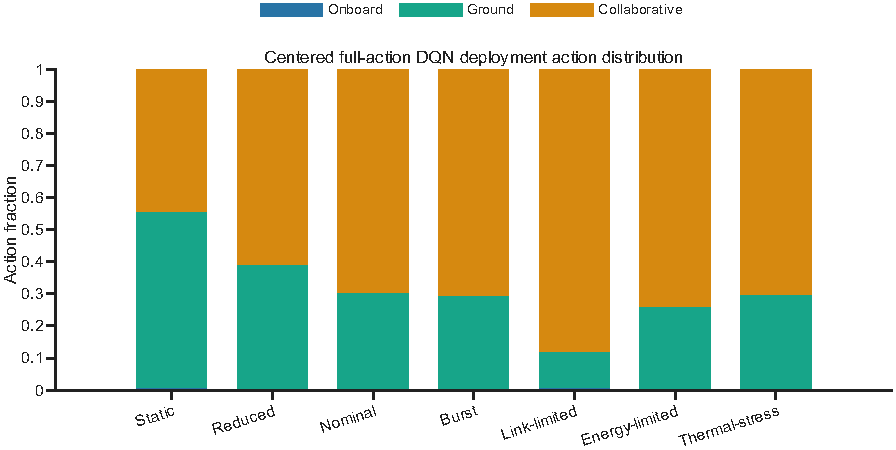
\includegraphics[width=0.90\textwidth]{figures/fig_reviewer_actions.pdf}
\caption{Mean deployment action fractions for \method under the physically coupled generator.}
\label{fig:actions}
\end{figure}

\section{Discussion and Limitations}

The revised evidence supports the complete MD-CBAD-DQN objective against a strictly matched standard-DQN backbone across five fully coupled regimes. Because the only algorithmic change is the centered all-action auxiliary loss, the comparison attributes the observed gain to the complete proposed training objective; it does not attempt to decompose that objective into additional intermediate methods. RL is not required for the static control: immediate minimization is exact when action-dependent carryover is removed, and four-step receding-horizon planning is strongest under weak coupling.

The planner comparison also bounds the motivation. MPC-4 uses the simulator transition model and perfect four-task forecasts, yet a short horizon underweights consequences persisting beyond four arrivals. Increasing $H$ raises enumeration from $3^4$ to $3^H$ and may improve planning, but we did not establish the best horizon or compare against approximate tree search, mixed-integer programming, or dynamic programming with discretized resources. We therefore claim an advantage over this transparent finite-horizon baseline, not over all traditional optimization.

The matched DQN backbone is an attribution design rather than a broad reinforcement-learning benchmark. Double DQN, dueling networks, prioritized replay, multi-step returns, noisy networks, and distributional value learning were intentionally excluded because adding them only to one arm would obscure whether the difference arose from CBAD. Accordingly, the evidence establishes an incremental effect of the complete auxiliary objective over standard DQN under matched conditions; it does not establish superiority over every enhanced value-learning method.

The new generator removes internally contradictory independent samples by deriving heat, energy, latency, and transmitted volume from common primitives. NASA and CCSDS sources bound selected engineering assumptions, while automated checks enforce data-flow inequalities. Nevertheless, the joint distribution is synthetic rather than fitted to mission telemetry. NASA itself cautions that component performance is mission-specific~\cite{nasa2026soa}. The sensitivity study covers only prespecified one-factor changes, not simultaneous uncertainty or structural model error.

Matched training components attribute the simulator-level difference to the complete auxiliary objective, but external validity remains limited. Preview outcomes are exact only under the specified deterministic simulator and may be biased onboard. The topology remains one satellite and one ground path, the action space contains only three modes, and inference remains simulation-based. Future work should use flight or hardware-in-the-loop traces, expand to multiple satellites and contacts, and compare scalable approximate planning at longer horizons.

\section{Conclusion}

We introduced \method to exploit simulator-exact one-step resource models while retaining the factual standard-DQN target and factual loss term. Under the physically coupled simulator, the complete CBAD objective improved on standard DQN across five fully coupled regimes and had the lowest mean among the evaluated deployment methods. A four-step rolling planner and coupling controls show that the observed benefit is confined to sufficiently persistent resource carryover.

\section*{Funding}

This work was supported by the National Key Research and Development Program of China under Grants 2022YFF0503904 and 2022YFD2401202. Additional support came from the Shenzhen Higher Education Institutions Stabilization Support Program under Grant GXWD\allowbreak20220811163556003. The National Natural Science Foundation of China supported this work under Grant 62202127, and the Shenzhen Natural Science Foundation under Grant JCYJ\allowbreak20241202123731040. Further support came from the Guangxi Science and Technology Base and Talent Special Project under Grant Gui Ke AD25069103.

\section*{Data and Code Availability}

The accompanying versioned repository contains the simulator, all 100 reviewer-revision checkpoints (60 primary and 40 preview-error models), raw evaluations, seed-level summaries, fixed-seed inference, direct Python dependencies, MATLAB figure source, and LaTeX-table generator under \texttt{md\_cbad\_dqn/}. The machine-readable \texttt{results/reviewer\_revision/validation.json} records expected row and checkpoint counts together with SHA-256 hashes of result artifacts. The command in the reproducibility subsection regenerates the complete result chain. A public archival DOI remains to be minted before publication; this manuscript does not imply that a permanent external archive already exists.

\begingroup
\small
\setlength{\itemsep}{0.2em}
\bibliographystyle{unsrt}
\bibliography{ref}
\endgroup

\end{document}
